\documentclass[letterpaper]{article}
\title{Final Project Time Log}
\date{}
\author{Jamie Maher, Joey Curci, James Farrington, Chris Rho}

\usepackage{graphicx}
\usepackage{hyperref}
\usepackage[margin=1in]{geometry}

\begin{document}
\maketitle
%------------------------------------------
\section*{Time Log}

The following table is the group's recorded time log

\begin{table}[h!]
\centering
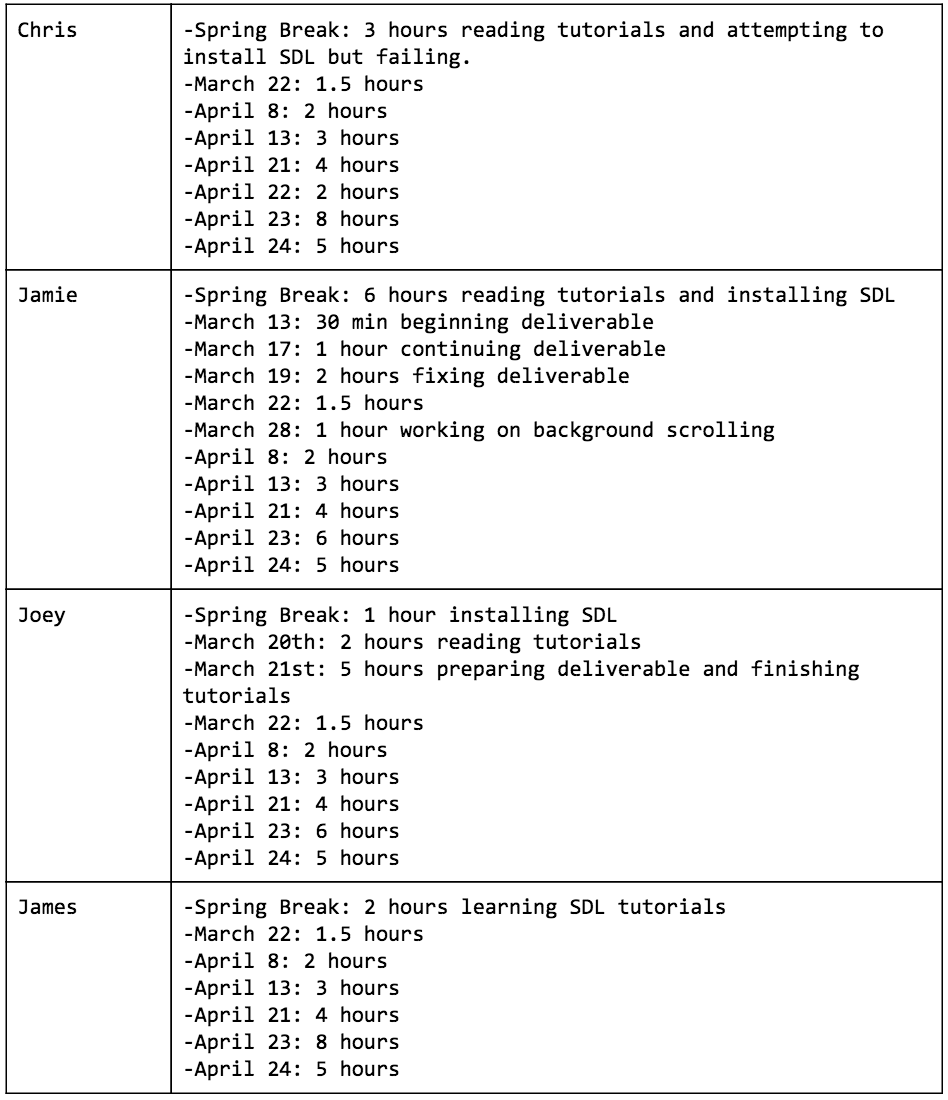
\includegraphics[width=5in]{table.png}
\caption{Group Time Log}
\end{table}
%------------------------------------------
\section*{Meeting Descriptions}

\subsection*{March 22:}
Met for an hour and a half to work on scrolling the background in the way that we would want. We decided to make a background class that would handle the right and left key events. We decided it would make the most sense to keep the Mario figure centered in the middle of screen, and just move the background behind it.

\subsection*{March 29th:}
Met for around 2 hours to work on how to implement level design and how to setup a basic main menu.  We decided that we wanted to have multiple enemies, including: goombas, koopas, and thwomps.  On this day we began the initial planning of the level and the main menu.

\subsection*{April 8th:}
We all met for 2 hours to work on creating the Goombas and handling coins as well. We began discussing how to have the goomba move properly and how the user would kill it.  We also got the map to work properly so we could begin designing the level more effectively.  Our task was to have the rendering of the goomba working.

\subsection*{April 13th:}
We all met for 3 hours to work on having the goomba move and having proper coin collection.  At this meeting we began thinking about how to implement multiple levels in our game, as well as what powerups to include.  We decided to only have coins and 1UP mushrooms.  At this meeting, we got the gooma to work properly and began to have hit collisions for the enemies.  We also added the koopa to the level and also worked on hit detection for the koopa. The last change we made was extending the level.

\subsection*{April 19th:}
Hours of hard work and dedication led to this shining moment: our pilgrimage to Blaze pizza.  Relationships grew as we feasted upon the glorious pizza.  We learned just as much about ourselves as we did about each other.  Together, we can do anything and this meeting was truly essential to this realization.  Just like how the battle of Stalingrad was the turning point in WWII, this meeting truly changed the tides of our project.

\subsection*{April 21st:}
We all met for 4 hours to discuss how to implement the mushrooms into the level.  We also worked on getting text to display the score and lives at the top.  At this meeting, we changed from having multiple levels to simply having one long level and focusing on the time and score.  We wanted to get high scores so you could compete with your previous bests.  Another enemy was added because we added the thwomp to the level.  

\subsection*{April 23rd:}
We all met for 5 hours to fix the jumping issue we had.  In addition, we fixed the collisions so enemies would die correctly.  We also began to implement sounds into the game.  The game was nearing completion so we decided to spend the time on fixing bugs and other errors in our code.  This led to the fixing of the jumping issue in which mario would not return to the proper height after landing.  This also fixed our enemy collisions.

\subsection*{April 24th:}
We all met again for 5 hours to add the finishing touches to our project.  We added more sound effects and began working on the report and presentation.

\end{document}